
\subsection{Experiment Setup}
\paragraph{Dataset:}
The study described in this paper uses datasets of South American Tweets, collected over 12 months (from May 2013 to May 2014), covering 22 countries. Our Twitter dataset was built from querying Datasift's streaming API. Tweets from GPS-enabled devices also report latitude/longitude coordinates. However the percentage of such Tweets in the collected sample was too low to be useful.

\paragraph{Geocoding:}
For this study, we build a geocoding tool to lookup each Tweet's location. To get a higher recall of geo-located Tweets, we apply our own geocoding library - that uses World Gazettee~\cite{worldgazetteer} database to lookup location names and geo-coordinates. For event geolocation we look into Tweet's text for string matches to location (cities, admin, country) and landmark place names such as Plaza de la Independencia (Quito, Ecuador). In cases, where no event location was found in Tweet's text, we use geo-coordinates or self-reported location string in Tweet's metadata.

Using above described pipeline, we were able to extract the geolocated $598,300$ cities from South American Twitter. Since many geolocated Tweets are really sparse within one day, we only consider the 1290 cities whose daily average Tweets larger than 100.

\paragraph{Major events labels:}
We focus on two kinds of major events, one is natural disasters, eg., earthquake, floods, and landslides, that we found from European Emergency Response Coordination Center(ERCC)~\footnote{http://erccportal.jrc.ec.europa.eu/} and World Top Stories Timeline~\footnote{http://www.mapreport.com/}; the second one is major social unrest events. We define major mass protest events by checking a gold standard report(GSR) in Latin America provided by MITRE.


\subsection{Group absenteeism detection results}
Using the geocoded Tweets as dataset, based on every day's Tweets volume, we calculate each city's Z-score. We set the time interval in two levels, a small-grained level (30 minutes), which is used to see if it connect with emergence events, the big-grained level is one day, which used to see if it associates with long-term events. When we set the time interval as half hour, then for half hour of that day, we calculate their respective Z-score(30) based on their previous 30 days' time slot Tweets count. For example, Jan 31, 2014's Z-score(30) at 8AM is got by previous 30 days Tweets counts at 8AM. If the time interval is one day, when calculate a weekday's Z-score(30), only use the previous 30 weekdays Tweets count to calculate. To calculate a weekend day's Z-score(30), only use previous 30 weekend days. The lowest absenteeism score means the most obvious absenteeism behavior. Set the test period from Jun 01, 2013 to May 31, 2014, for each day, employ the algorithms described above, and select the most absenteeism group of that day. For the one day time interval, each day will get one absenteeism group; for the 30 minutes time interval, will get 48 absenteeism groups for every half an hour, we pick the lowest group score.


After get a whole year absenteeism groups of each day, then we try to discover what events are going on of those absenteeism groups. How to decide whether an absenteeism group associate with major events? Of each absenteeism group, if there is one city coincide with the major events area, we take it as associated with the major events.
%Of the whole year absenteeism groups, not all the selected groups have major events, sometimes it is difficult to decide if they associate with major events.
Compared with the ERCC and GSR records, we list 17 groups which associate with major events, in Table~\ref{table:list_events}.

On Jun 20, 2013, set time interval as one day, for regional algorithm we set $A$ as 0.02, and for subgraph algorithm, we set $d_{th}$ as 0.1, we get two set of absenteeism groups which associate with Brazil spring events, plotted in Figure~\ref{fig:20130620}. With the same setting, we also plot the absenteeism groups on May 01, 2014, which shows the central America Labor Day's group absenteeism distribution, see Figure~\ref{fig:labor_day}.

On Sep 11, 2013, using subgraph algorithm, we found the absenteeism group at 15:00 is the lowest. By checking the GSR record, we find on Sept 11, 2013, there were 17 cites in Mexico having protests demonstration. Using the minimal weight graph algorithm, of the selected 20 absenteeism cities, 6 of them involved in the teachers' protest events. This shows huge protest events can result in high group absenteeism phenomenon.


\begin{figure}[t]
	\centering
	\subfigure[regional]{
		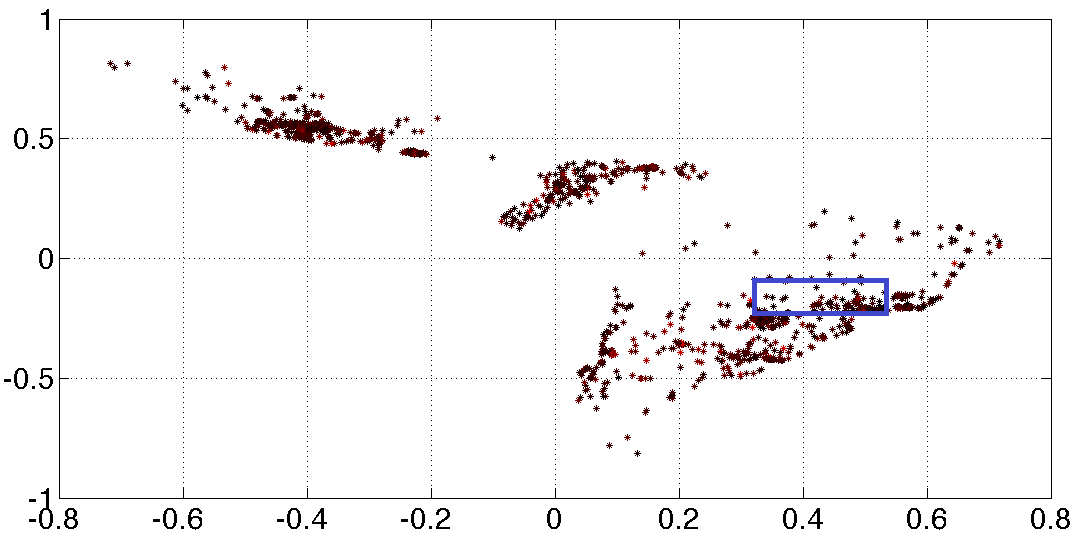
\includegraphics[width=1.55in,height=1.55in] {figures/Brazil_regional_20130620.png}
		\label{fig:Brazil_regional_June20}
	}
	\subfigure[subgraph]{
		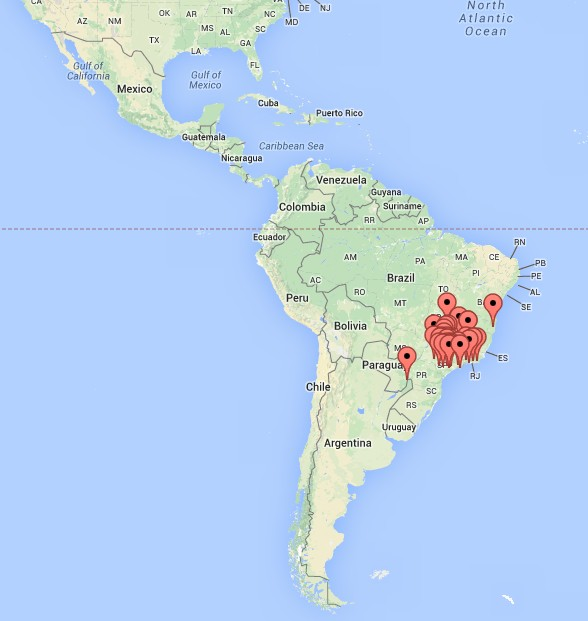
\includegraphics[width=1.55in,height=1.5in] {figures/Brazil_subgraph_20130620.jpg}
		\label{fig:Brazil_subgraph_June20}
	}
	\vspace{-1em}
	\caption{ The selected absenteeism group in South American on June 20, 2013.}
	\label{fig:20130620}
\end{figure}

\begin{figure}[t]	
	\centering
	\subfigure[regional]{
		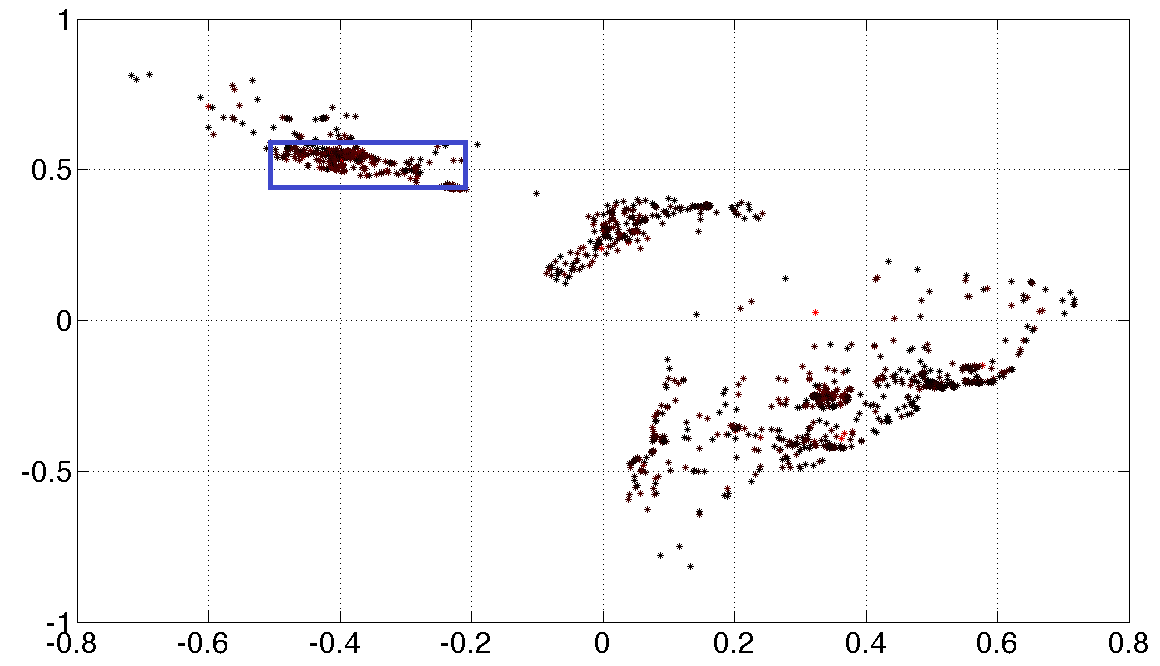
\includegraphics[width=1.55in,height=1.55in] {figures/regional_labor_day.png}
		\label{fig:Mexico_regional}
	}
	\subfigure[subgraph]{
		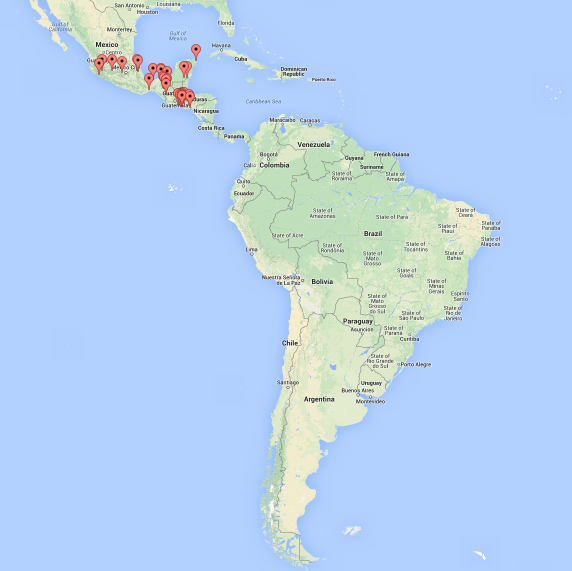
\includegraphics[width=1.55in,height=1.5in] {figures/subgraph_labor_day.png}
		\label{fig:Mexico_subgraph}
	}
	\vspace{-1em}
	\caption{ The selected absenteeism group in South American on May 1st, 2014.}
	\label{fig:labor_day}
\end{figure}


\subsection{Comparison of different algorithms}
We use the data set on February 27, 2014, and set the time window as one day. We plot the comparison results from two aspects:  running time complexity, and parameter sensibility in figure~\ref{fig:performance},~\ref{fig:running_time},~\ref{fig:sensibility}.
\begin{figure}[h]
	\centering
	\subfigure[regional]{
		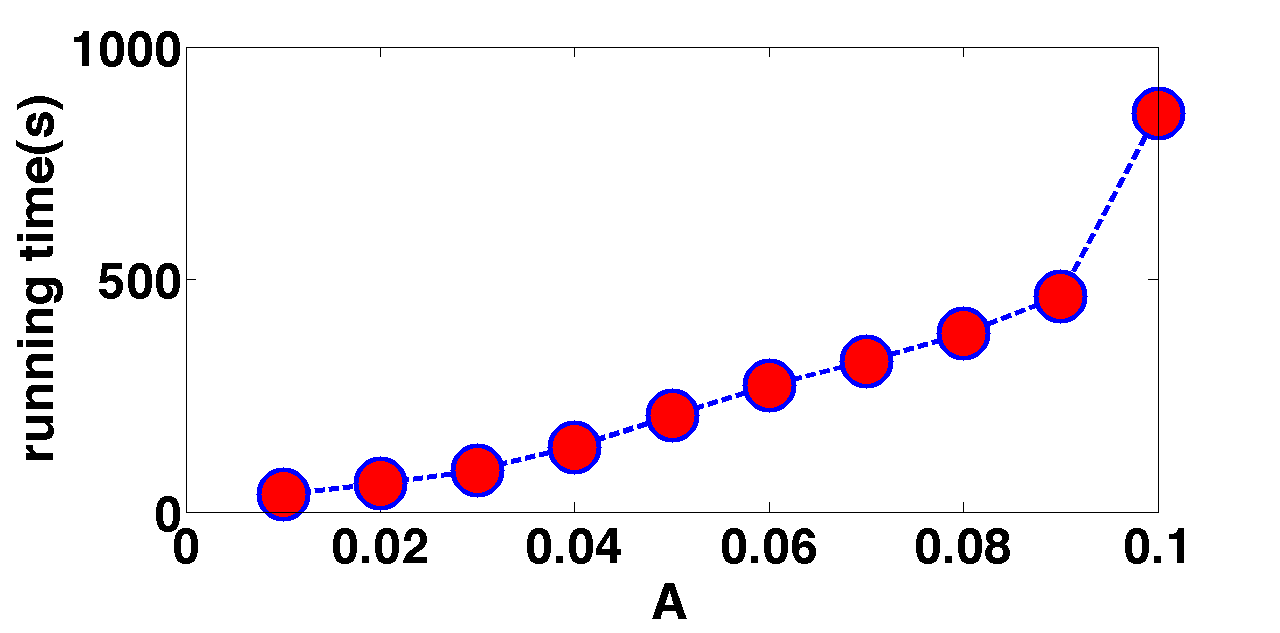
\includegraphics[width=1.55in,height=1in] {figures/performance1.png}
		\label{fig:performance1}
	}
	\subfigure[ubgraph]{
		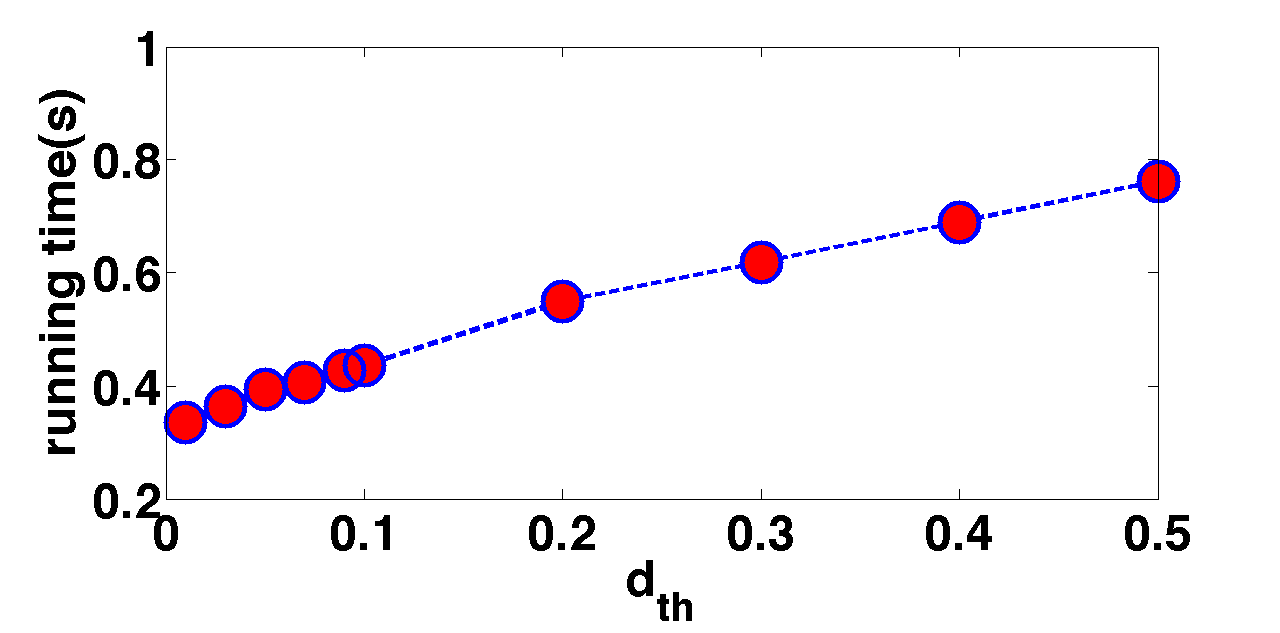
\includegraphics[width=1.55in,height=1in] {figures/performance2.png}
		\label{fig:performance2}
	}
	\vspace{-1em}
	\caption{running time vs input parameter.}
	\label{fig:performance}
\end{figure}
\paragraph{Running time}From Figure~\ref{fig:performance}, we can see that the running time of regional approach increases extremely fast when $A$ is larger than 0.09. While in subgraph approach, the increasing speed is much stable as $d_{th}$ increases. This is because regional approach's time complexity is in proportion to $A^2$, while subgraph approach's time complexity is proportional to $d_{th}$. From Figure~\ref{fig:running_time}, we can see clearly that for the regional algorithm, the running time complexity also increase sharply with the input size $n$, while in subgraph approach, the increase speed is moderate. This is because the regional approach's timing complexity is $O(N^3)$, while subgraph approach's time complexity is $O(N^2)$. Thus, the subgraph approach is better  than regional approach in term of running time for a larger absenteeism group.
\begin{figure}[h]
	\centering
	\subfigure[regional]{
		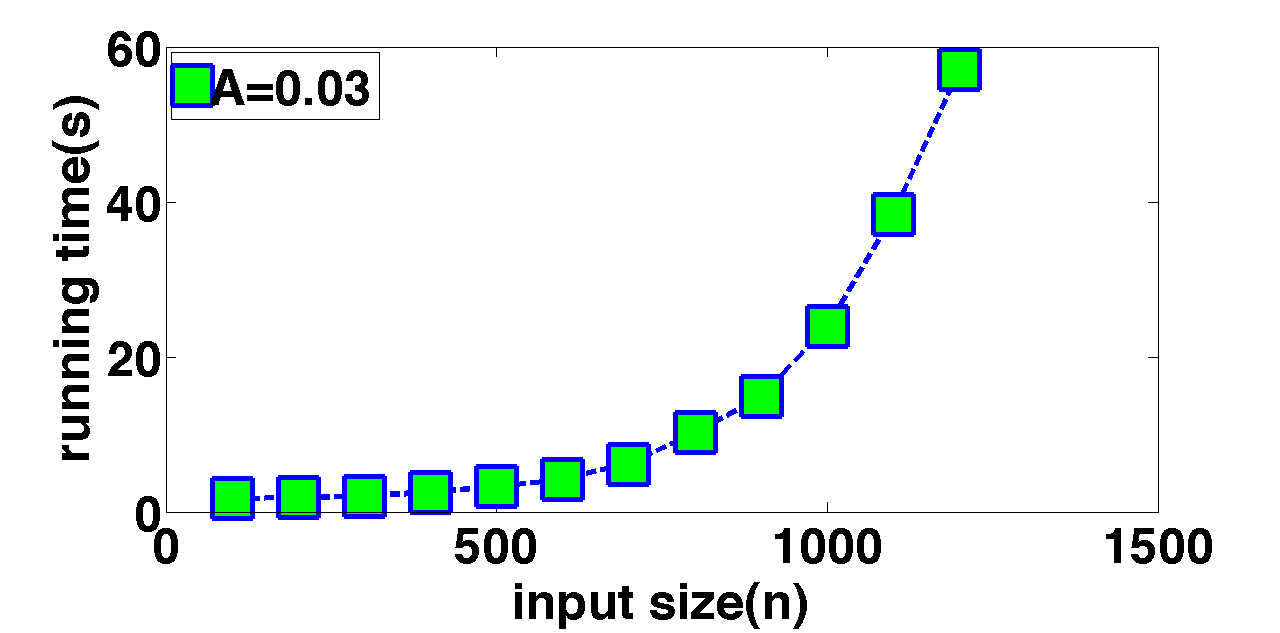
\includegraphics[width=1.55in,height=1in] {figures/running_time1.png}
		\label{fig:running1}
	}
	\subfigure[subgraph]{
		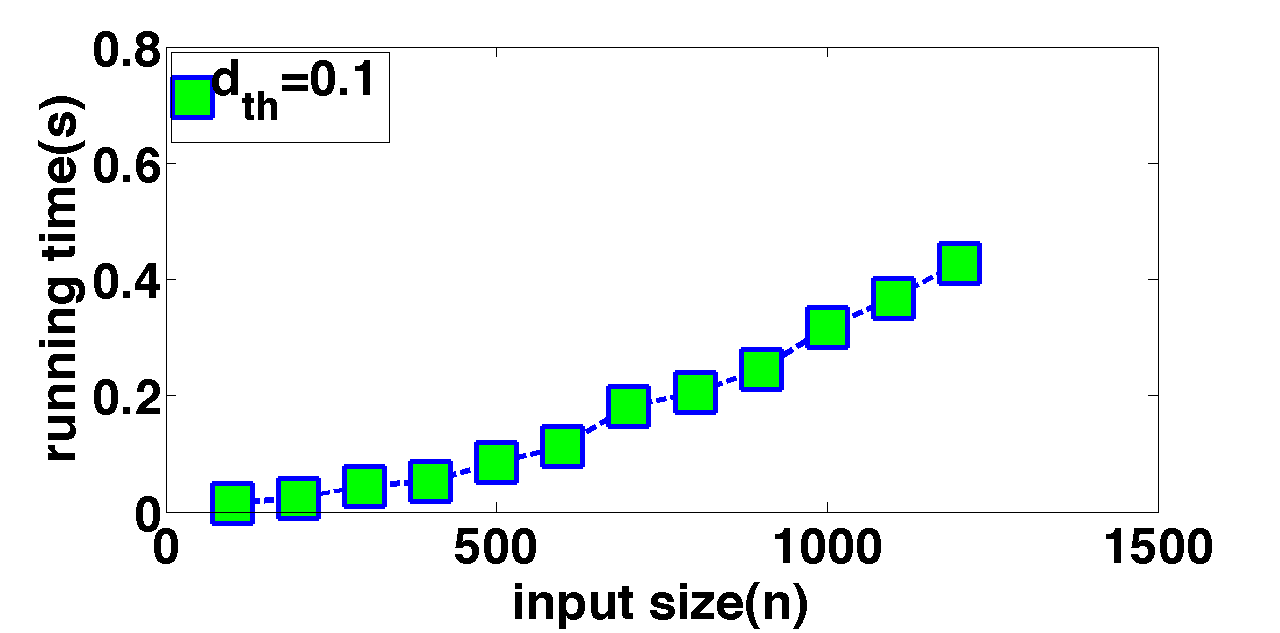
\includegraphics[width=1.55in,height=1in] {figures/running_time2.png}
		\label{fig:running2}
	}
	\vspace{-1em}
	\caption{Running time vs input size.}
	\label{fig:running_time}
\end{figure}
\paragraph{Parameter sensibility}In regional approach, set the input parameter as $A$, and the optimal absenteeism group as $P_{min}$. When $A$ is changed to $A$', the optimal absenteeism group is changed to $P_{min}$, define the output error as the city number that exists in $P_{min}$ but not in $P_{min}'$, and denoted as $P_{min}-P_{min}'$. We define the parameter sensibility as: $$sensibility=\frac{{|P_{min}-P_{min}'|}/{|P_{min}|}}{|A-A'|/{A}}.$$ We plot the regional approach and subgraph approach's sensibility in Figure~\ref{fig:sensibility}. In the regional approach, when the input parameter error is smaller than 20\%, the output absenteeism group error is less than 5\%. While in the subgraph approach, the output absenteeism group error is linear to the input error parameter. This is probably because regional approach aggregates all the absenteeism score covered by the region, and usually has a much larger city number than the subgraph approach, and makes regional approach better at anti-noise.  All in all, the regional algorithm focuses on all the cities in the cover group, and has a better global performance at anti-noise, while is inferior to the subgraph counterpart in term of running time complexity.
\begin{figure}[h]
	\centering
	\subfigure[regional]{
		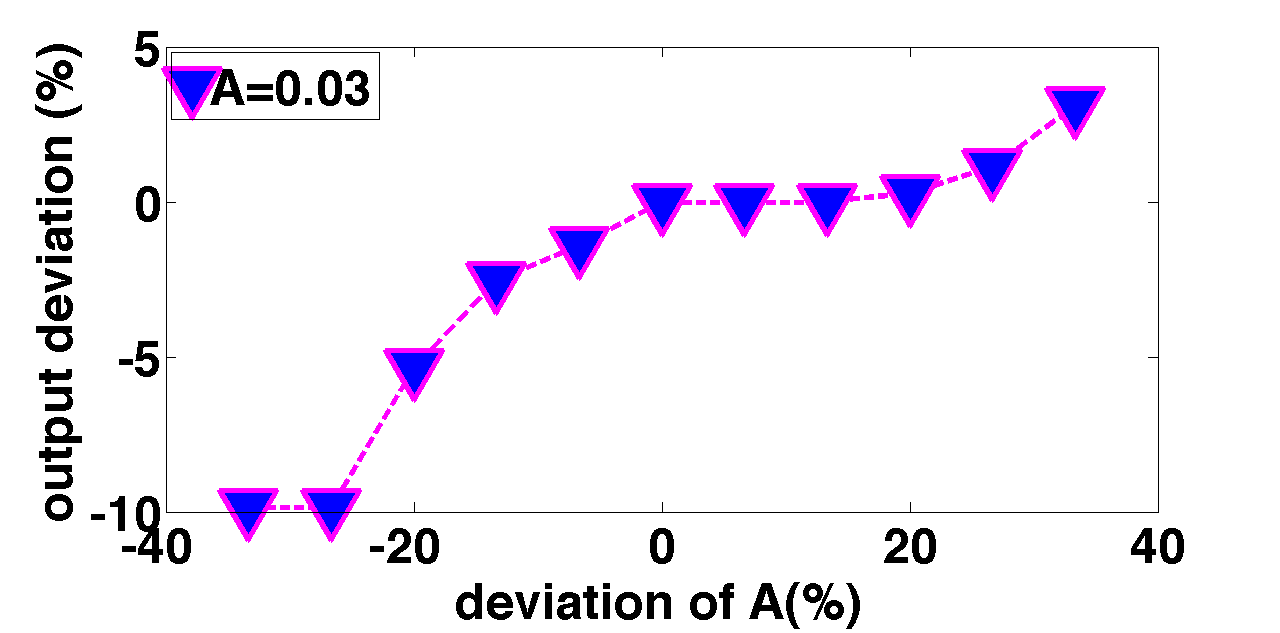
\includegraphics[width=1.55in,height=1in] {figures/sensibility1.png}
		\label{fig:sensibility1}
	}
	\subfigure[subgraph]{
		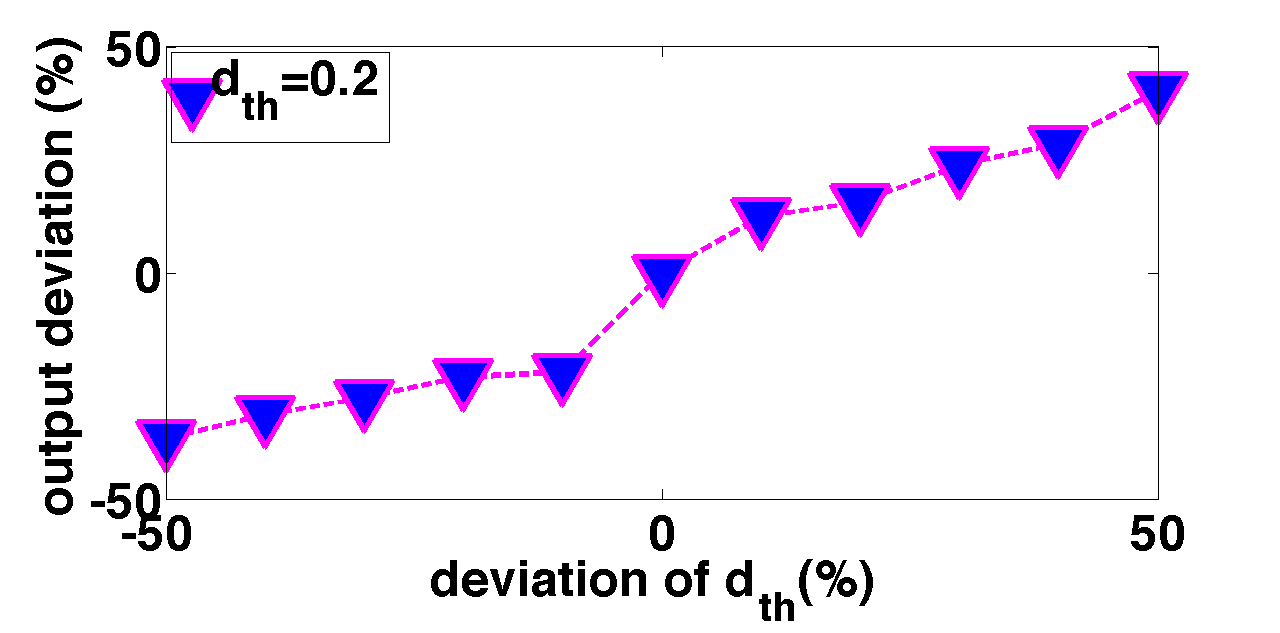
\includegraphics[width=1.55in,height=1in] {figures/sensibility2.png}
		\label{fig:sensibility2}
	}
	\vspace{-1em}
	\caption{Sensibility comparison of the two algorithms.}
	\label{fig:sensibility}
\end{figure}

\subsection{Absenteeism case study}
\subsubsection{What caused absenteeism?}
To retrospect what caused the group absenteeism is never a trivial task,  because there are so many factors that might affect whether people post Tweets or not, and how frequent they post Tweets. Generally, the absenteeism of Tweets can be explained at leaf of the two aspects.

\paragraph{Population mobility}
The population at one location is not a constant, which can vary at different time. As shown in Fig~\ref{fig:holidays_brazil}, We plot the Tweets of 131 cities in Brazil based on the weekdays and holidays from June 2013 to May 2014. From Figure~\ref{fig:holidays_brazil}, we can see that usually Friday features the lowest Tweets volume, and holiday also has a low Tweets volume, but has the highest deviations. Take the example of Chetumal, Quintana Roo, Mexico on May 1st, whose absenteeism score is $-3.00$. For the day of May 1st, which happens to be Labor Day of Mexico, large amount of people go out for travel, resulting in absenteeism in the local town.
%\begin{figure}[h]
%	\centering
%	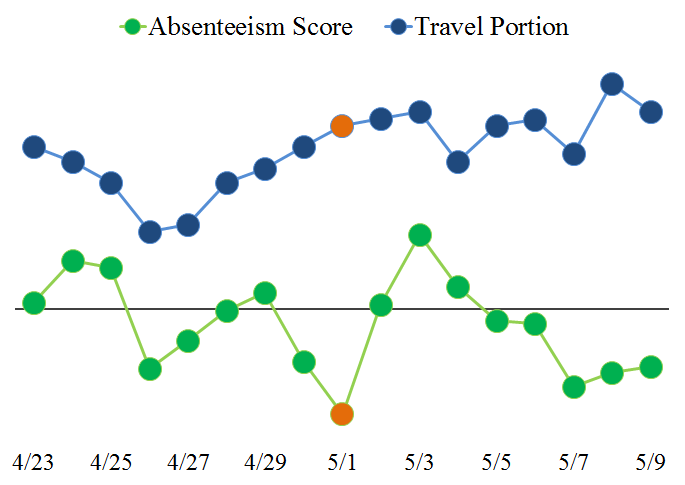
\includegraphics[width=1.8in, height=1in]{figures/userid_portion.png}
%	\caption{Absenteeism score correlate with people's travel portion, in Chetumal, Quintana Roo, Mexico, from Apr-23-2014 to May-09-2014. The orange circle shows on May-01-2014 (the national holiday), the deepest absenteeism score corresponding to a higher travel portion.
%	}
%	\label{fig:userid}
%\end{figure}

\begin{figure}[h]
	\centering
	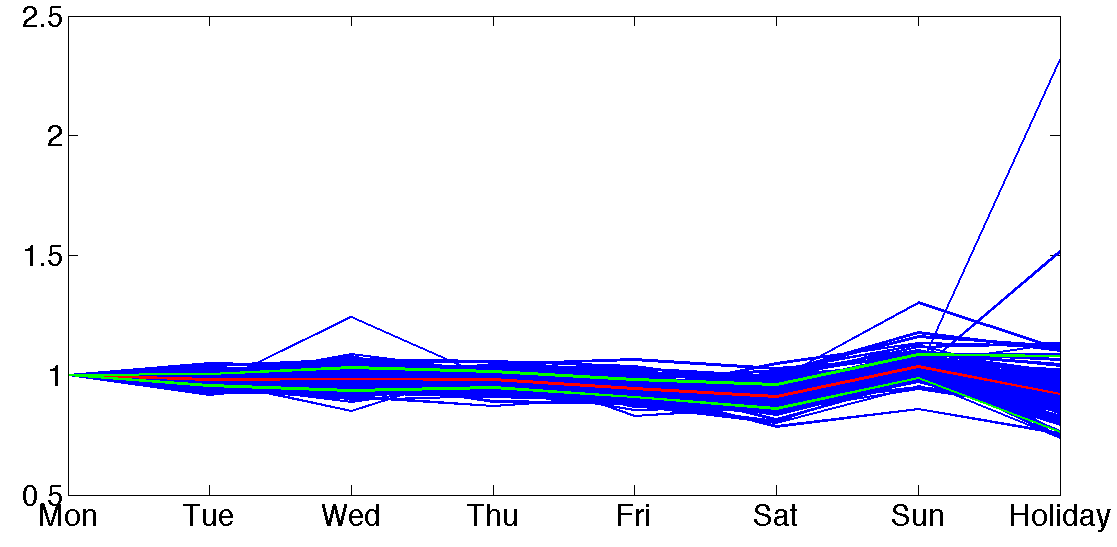
\includegraphics[width=2in]{figures/HolidayCurve_Brazil.png}
	\caption{Tweets daily volume of 131 cities from June 2013 to May 2014. Each day's volume is normalized by Monday's average value. The red line represents the $mean$ value, and the green lines represent the $mean\pm \sigma$ boundaries.
	}
	\label{fig:holidays_brazil}
\end{figure}

\paragraph{Major (negative) events}
Tweets rate is heavily depends on people's social activities, especially when major negative events happen. For instance, at 15PM on Sep 11, 2013, Mexico, a large portion of people were involved in protest that they have no time to Tweet, which results in Twitter absenteeism from 15:00 to 15:30. Tweets rate is also closely depends on people's sentiment, for instance, on Jan 31, 2014, Chile'S IPSA stock index hit lows not seen in over 4 year, people might not like to Tweet. Even weather has a close relationship with the Tweets number. Usually, a good weather introduces more topic for people. Otherwise, severe weather like heavily storms which result in floods usually hinder people from doing any entertainment, and the Tweets number will drop down, as shown in table~\ref{table:list_events}.

\subsubsection{Why use group absenteeism?}
\paragraph{Irreplaceable}The unique of absenteeism signal made it plays a special role in event detection. For instance, on May 16, 2014, when the anti-World cup protest happened on cities Rio de Janeiro and Sao Paulo, large portion of people walked on the street for protest, both cities' Tweets absenteeism score reach the lowest point, see Figure~\ref{fig:World_cup}. Also the case of Brazil floods on Dec 12, 2013 is the same situation, when heavy rains caused floods, while the floods get more and more severe, the Tweets tends to be inactive, and on the day of Dec 24, the floods was the worst day, while at the same time, the Twitter at local state reached the lowest absenteeism score, see Figure~\ref{fig:Brazil_flood}. In the two cases, using burst algorithm cannot identify such events by only observing Twitter burst activity.

\begin{figure}[h]
	\centering
	\subfigure[]{
		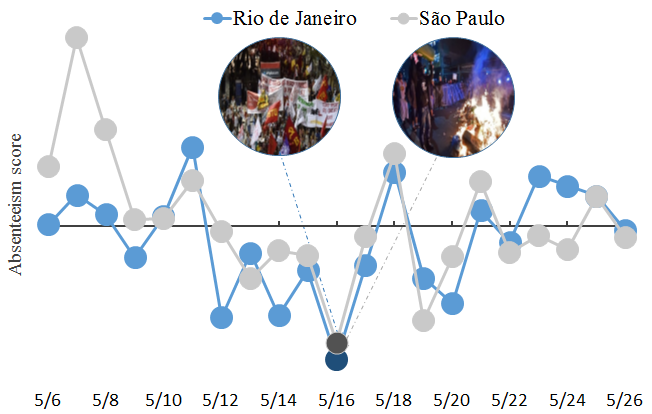
\includegraphics[width=1.55in,height=1in] {figures/Worlp_cup_example1.png}
		\label{fig:World_cup}
	}
	\subfigure[]{
		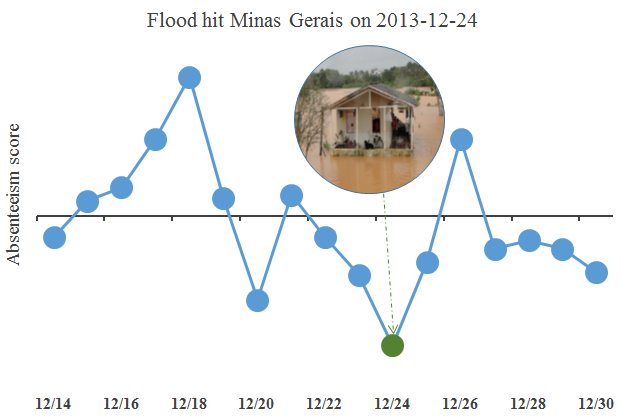
\includegraphics[width=1.55in,height=1in] {figures/flood_example.png}
		\label{fig:Brazil_flood}
	}
	\vspace{-1em}
	\caption{ (a) Tweets Absenteeism score in two cities of Brazil while they are proceeding anti-world cup protest on May-16-2014. (b) Tweets Absenteeism score reach the lowest point when floods hit Minas Gerais, Brazil on Dec-24-2013.}
	\label{fig:flood_cup}
\end{figure}

\paragraph{Earlier signal}
Take the case of Apr 01, 2014 Chile earthquake for instance, when the earthquake erupted at 20:46 local time, the Twitter appears a strong group absenteeism signal at the very first 4 minutes, after that, Twitter started to burst. Using the subgraph algorithm, when the time window set enough small, it can capture the group absenteeism much earlier than the later burst signal. We can see using very small-grained time interval, employing the absenteeism algorithm is able to capture the abnormal Twitter activity earlier, especially when facing emergence events.
\begin{figure}[h]
	\centering
	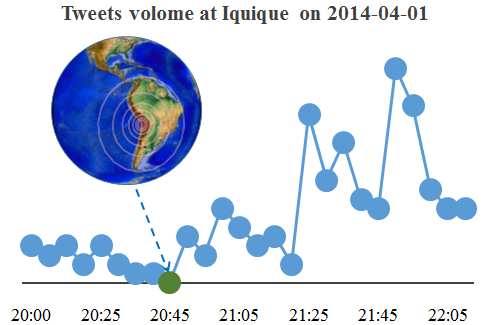
\includegraphics[width=1.8in, height=1.1in]{figures/earthquake_example.png}
	\caption{Tweets volume at Iquique, Tarapacá, Chile on Apr-01-2014. After the M8.2 earthquake erupt, in 4 minutes, the geocoded Tweets at Iquique is 0.
	}
	\label{fig:earthquake}
\end{figure}


% % % % % % % % % % % % % the end% % % % % % % %
%
%\subsubsection{What caused absenteeism?}
%To retrospect what caused the group absenteeism is never a trivial task,  because there are so many factors that might affect whether people post Tweets or not, and how frequent they post Tweets. For simplicity, we model the Tweets volume of city $c$ on day $d$ as the following function:
%\begin{equation}
%  \label{eq:3D_distance}
%  \begin{array}{l}
% 	\mathcal{TW}(c,d) = \mathcal{M}*\beta
%  \end{array}
%\end{equation}
%$\mathcal{M}$ is the Twitter user number, and $\beta$ is the average Tweets number that one user post in time unit. According to this mechanism, the absenteeism of Tweets can be explained at leaf of the two aspects.
%
%\paragraph{User number $\mathcal{M}$}
%Usually, $\mathcal{M}$ is not constant, and varies at different time. As shown in Fig~\ref{fig:holidays_brazil}, We plot the Tweets of 131 cities in Brazil based on the weekdays and holidays from June 2013 to May 2014. From Figure~\ref{fig:holidays_brazil}, we can see that usually Friday features the lowest Tweets volume, and holiday also has a low Tweets volume, but has the highest deviations. Take the example of Chetumal, Quintana Roo, Mexico on May 1st, whose absenteeism score is $-3.00$. For the first event day is May 1st, which happens to be Labor Day of Mexico, large amount of people go out for travel, resulting in absenteeism in the local town.
%\paragraph{Tweets rate $\beta$}
%Tweets rate is heavily depends on people's social activities. For instance, at 15PM on Sep-11-2013, Mexico, a large portion of people were involved in protest that they have no time to Tweet, which results in Twitter absenteeism during this time slot. Tweets rate is also closely depends on people's sentiment, for instance, on Jan-31-2014, Chile'S IPSA stock index hit lows not seen in over 4 year, people might not like to Tweet. Even weather has a close relationship with the Tweets number. Usually, a good weather introduces more topic for people. Otherwise, severe weather like heavily storms which result in floods usually hinder people from doing any entertainment, and the Tweets number will drop down, as shown in table~\ref{table:list_events}. 